
\section{Social media submissions}
\label{data_reddust}
%\subsection{Introduction}

Reddit is a popular social media platform for discussing a wide range of topics. It has become an prominent source of information for data analysis on social media as it provides an abundance of data with rich structure and covers a broad range of topics. Such data has many applications, including personalizing healthcare \cite{gyrard2018personalized}, recommendations, search, and conversational agents. 
Reddit is used by approximately 330 million users\footnote{ \href{https://redditblog.com/2018/11/13/holiday-on-reddit}{https://redditblog.com/2018/11/13/holiday-on-reddit}}
with 2.8 million comments written each day\footnote{ \href{https://www.digitaltrends.com/social-media/reddit-ads-promoted-posts}{https://www.digitaltrends.com/social-media/reddit-ads-promoted-posts}}. 

Despite its popular and abundant data, few have considered Reddit as a source of data for inferring users' personal traits. However, many Reddit submissions contain a sufficient amount of personal information; an exemplary submission, indicating the user's hobby, is shown in Figure \ref{fig:input}. Prior work has focused on Reddit merely as a source of demographic information, whereas rich attributes, like \textit{profession} and \textit{hobby}, are usually overlooked. 

\begin{figure}[th!]
\centering
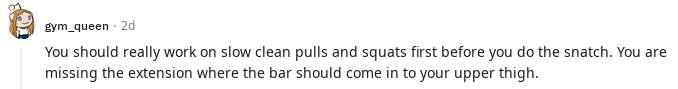
\includegraphics[width=0.85\textwidth]{data/pics/gym_queen.png}
\caption{
Example of a Reddit comment.
%Cues in bold suggest \emph{brewing} as the user's hobby.
}
\label{fig:input}
\end{figure}

We address this gap by creating a labeled dataset of Reddit users %\footnote{Available at {\scriptsize \url{http://pkb.mpi-inf.mpg.de}}.}
(including their posts and comments) that covers five user attributes: \textit{profession, hobby, family status, age,} and \emph{gender} \cite{tigunova2020reddust}. The collected submissions can be used as a proxy for dialogue utterances in conversational data research.
%We leveraged three high-precision approaches to identify predicates and their object values in users' posts: \textit{(1)} natural language patterns matching assertions like \textit{I am a flight attendant}, \textit{(2)} bracket patterns matching structured assertions of users' ages and genders (\textit{I [35m] just broke up with my girlfriend}), and \textit{(3)} flair metadata specific to particular subfora. We used human judgments to validate the high-precision nature of these approaches before performing an analysis of the resulting dataset. 

\subsection{Related work}

Automatic methods for identifying users' personal attributes 
from social media focus on user-generated content from Twitter, with a few exceptions that explore Facebook \cite{sap:EMNLP14,Schwartz2013PersonalityGA} or Reddit \cite{fabian2015privacy,finlay2014age,gjurkovic-EtAl:2018} posts.
Such methods, particularly supervised learning approaches, require a collection of user-generated content labelled with personal attributes of interest.

Data collection for such models is mostly done via: manual annotation after a focused search with specific keywords or hashtags \cite{pietro:ACL15,Rao:2010}, public profile linked to Twitter profile description \cite{burger:EMNLP11,flekova:ACL16:long}, self-reports as part of an online survey \cite{finlay2014age,flekova:ACL16:long,pietro:ACL17:long,pietro:COLING18,sap:EMNLP14,schwartz2013personality}, or pattern-based extraction approach 
(e.g., \texttt{\small(I$|$i) (am$|$'m$|$was) born in + number (1920-2013)}) on user profile description or user posts \cite{fabian2015privacy,kim:ACL17:short,sloan2015tweets,tigunova2019listening}.
Several works \cite{basile:2017,bayot:MOD17} made use of labelled datasets published within the shared task on author profiling organized by the CLEF PAN lab \cite{stein:2017o,stein:2017l}. 

There has been less effort on identifying demographic attributes of Reddit users compared with the body of work that exists for Twitter users. However Reddit posts have been exploited for other purposes, such as determining \emph{users' personality} \cite{gjurkovic-EtAl:2018}, \emph{mental health condition} \cite{cohan2018smhd}, \emph{domestic abuse} \cite{schrading2015analysis} and \emph{irony detection} \cite{wallace2014humans}, among others.
\citet{thelwall2018she} investigate how the topic of subreddit influences the gender ratio within it. The study was performed on 100 subreddits grouped by interest; gender information about the users was collected by guessing it from their usernames, which is arguably a low-precision strategy. Smaller scale Reddit datasets exist for \emph{gender}, \emph{age} and \emph{location} attributes \cite{fabian2015privacy,finlay2014age}, which are unfortunately not publicly available. As far as we know, we are the first to consider \textit{hobby} as a personal attribute of interest to be identified from online communication.

\subsection{Background}

%Reddit\footnote{{\scriptsize \url{https://www.reddit.com/}}} is a social news website and forum where registered members can submit content including links, text posts, and images, which are then voted up or down by other members.
%Before elaborating on the creation of our dataset derived from Reddit posts, we describe several concepts on Reddit that are relevant for the data collection process.

\paragraphHd{Posts and Comments.}
Discussions on Reddit are organized in threads, which are initiated by an original \textit{post} and may contain \textit{comments} replying to the post and to the other comments. This creates a hierarchical structure that resembles a conversation between the users.
Both posts and comments can be a textual content, a link with anchor text or images.

\paragraphHd{Subreddits.}
Reddit is organized into subreddits, which are fora that focus on specific topics.
Those can be split by interest (sports, politics, etc), by country or community, type of content (text, gifs, videos), and so on. Subreddits have their own rules, but any registered user can create them. By convention, subreddits are prefixed with \texttt{\small /r}. For example, users discuss hockey in the \texttt{\small /r/hockey} subreddit.

\paragraphHd{Flairs.}
Flair is a user or post metadata that is a unique feature of Reddit. Flair is a small image with a short text description that is attached to a post or a username. Flairs can be defined differently for specific purposes by each subreddit. For example, in \texttt{\small /r/travel} subreddit they may indicate the \textit{country} of the user, \textit{gender} in \texttt{\small /r/AskMen} and \texttt{\small /r/AskWomen} or users' \textit{favorite teams} in \texttt{\small /r/hockey}.
Flairs for posts can be useful to filter and search for a particular content.

\subsection{RedDust dataset}

In this section we describe the creation of our proposed \emph{RedDust} dataset, containing a collection of Reddit users. Each user in the dataset is associated with posts and comments they produce (which we call \textit{submissions} in the following) and users' inferred personal attributes.
We considered five personal attributes including \textit{gender}, \textit{age}, \textit{family status}, \textit{profession} and \textit{hobby}.
The dataset is created from the openly published \gls{Reddit dump}\footnote{ \href{https://files.pushshift.io/reddit}{https://files.pushshift.io/reddit}}, which spans between 2006 and 2018. 

There are several criteria on which users and submissions are included in RedDust, i.e., users who posted between 10 and 100 submissions, and submissions containing between 20 and 100 terms after filtering. We filtered out hyperlinks and user mentions (i.e., \texttt{\small @nickname}) from the original content.

Some subreddits are likely to contain many false positives, such as those concerned with video games or role playing. This leads to personal assertions talking about the users' projected persona in a particular context (e.g., \textit{``I am a priest looking for a guild''}). To mitigate this source of false positives, we blacklisted subreddits about gaming, fantasy and virtual reality from the top 500 subreddits sorted by the number of unique users. Posts made to blacklisted subreddits were discarded. 
Similarly, we discarded posts that contain quotations in order to reduce the possibility of the user referring to a third person (\textit{``... and he shouted `Hands on the counter, I am a cop!' ''}).

For attributes that usually have a unique value (i.e., \textit{gender}, \textit{age} and \textit{family status}) we also exclude users who state multiple different values to avoid introducing false positives. Meanwhile, we allow each user to have multiple attribute values for \textit{profession} and \textit{hobby}. The age of a given user is calculated relative to his or her age when writing the most recent comment. In the following we discuss particular techniques used to extract values for each personal attribute.

\subsubsection{Gender}
Gender has been the most popular user attribute to predict in existing user profiling work, particularly on Reddit \cite{fabian2015privacy,thelwall2018she,Vasilev2018}.
In 
RedDust
we consider gender as a binary predicate (\emph{female} or \emph{male}) 
as has been done in prior work. 

Instead of considering usernames as a means for gender classification, as was done by \citet{thelwall2018she}, we look for self-reported gender assertions, which provide labels of higher precision.
Specifically, we identified 
users' gender
using the following methods:
\begin{itemize}
    \item \textbf{Natural language patterns}.
    Following \citet{fabian2015privacy}, we manually created a set of patterns that indicate a specific gender. They have the general form of \texttt{\small (I am|I'm) a? <gender indicator>}, meaning that matches should contain `\textit{I am}' or `\textit{I'm}', optionally followed by an article `\textit{a}', then a word that indicates gender like `\textit{man}' or `\textit{mother}'. A comprehensive list of patterns we used is given in Table \ref{pat_table}, and the indicative gender words are shown in Table \ref{word_table}. Although the gender of a given user can be expressed in a longer snippet like ``\textit{I am a great mother}'', we do not allow extra words like \textit{great} to appear before gender-indicating words. This reduces false positives from statements like ``\textit{I'm a far cry from my mother}''.
    
    \item \textbf{Bracket patterns}.
    In certain situations, users often volunteer to indicate their demographic information in order to give their posts more context (``\textit{I [30f] was dating this guy [35m]...}'').
    This is common in relationship-related subreddits, where the users' age and gender are often relevant to the discussions. These cues are generally written in round or square brackets. To reduce false positives, we do not consider such patterns when they appear without brackets. To capture gender and age expressed in this way, we look for patterns of the form \texttt{\small (I|I'm|me) [<number>(m|f)]}.
    
    \item \textbf{Flairs}.
    Like \citet{Vasilev2018}, we also consider gender-indicating flairs attached to users.
    This logic is subreddit-specific, so we restrict ourselves to common subreddits.
    For example, in subreddits \texttt{\small /r/AskWomen} and \texttt{\small /r/AskMen} the flair is one of \textit{male, female, trans}, and so on, whereas in \texttt{\small /r/tall} and \texttt{\small /r/short} the flair is either \textit{pink, blue}, or \textit{other}.

\end{itemize}

\subsubsection{Age}
We label users' posts with age predicate using similar techniques as for gender:

\begin{itemize}
    \item \textbf{Natural language patterns}.
    To infer users' age, we utilized five patterns listed in Table \ref{pat_table}, with pattern (v) specifically designed to avoid false positives as in ``\textit{I am 6 feet tall}''.
    We then calculated the exact age for patterns (i)-(iii) by subtracting the birth year from the publishing year of the post containing such patterns.

    \item \textbf{Bracket patterns}.
    Numbers indicating age were jointly collected along with gender, as described in the above-mentioned bracket patterns for gender.
\end{itemize}

Finally, we made sure that the obtained ages for users in RedDust are within the range of 10-100 years old, since users under 13 are not allowed to register and there are unlikely to be many users above 100 years old.
This is helpful for reducing false positives, such as those in conditional sentences (``\textit{as if I were 5 years old}'').

\subsubsection{Family status}

We consider family status as a binary predicate indicating whether a person is \emph{single} or has a \emph{partner}. Similar to labeling gender, we relied on natural language patterns containing indicative words, which are detailed in Table \ref{pat_table} and \ref{word_table}, respectively. We distinguished two cases of indicative words: (i) \textit{{self-status indicator}}, used when the speaker refers to her own status (\emph{``I am divorced''}); and (ii) \textit{{partner indicator}}, when the speaker refers to the existence of a partner (\emph{``My boyfriend''}).

We additionally collected matches of negated patterns of both (i) and (ii)
%,i.e.,\texttt{\small I am not <self-status indicator>} and \texttt{\small I don't have a  <partner indicator>}
in order to expand the labelled data. Furthermore, given that the indicator word \emph{single} is often used in a more general context (e.g., `\emph{single player}', `\emph{single bed}'), we restricted the patterns containing this particular word, so that it should be immediately followed by punctuation, conjunctions or few allowed words like `\emph{father}'.

\begin{table*}[t!]
\centering
\begin{adjustbox}{width=0.88\textwidth}
\begin{tabularx}{\linewidth}{ll}
\toprule
\textbf{attribute} & \textbf{pattern(s)} \\
\midrule
gender & \texttt{\footnotesize (I am|I'm) a? <gender indicator>} {\footnotesize(e.g., \emph{man}, \emph{mother})} \\ [0.8ex] 
age & (i)\quad \texttt{\footnotesize I (was|am) born in <four digit year>} \\ 
 & (ii)\quad \texttt{\footnotesize I (was|am) born in <two digit year>} \\
 & (iii)\quad \texttt{\footnotesize I was born on <day, month, year>} \\
 & (iv)\quad \texttt{\footnotesize I am <number> years old} \\
 & (v)\quad \texttt{\footnotesize I am <number>} {\footnotesize immediately followed  by punctuation or conjunction} \\ [0.8ex]
family status & (i)\quad \texttt{\footnotesize I am <self-status indicator>} {\footnotesize (e.g., \textit{divorced}, \textit{single})} \\
 & (ii)\quad \texttt{\footnotesize (my|I have a) <partner indicator>} ({\footnotesize e.g., \textit{wife}, \textit{boyfriend})} \\ [0.8ex]
profession & \texttt{\footnotesize (I am|I'm) a <profession name>} \\ [0.8ex]
hobby & \texttt{\footnotesize <phrase indicator>} {\footnotesize (e.g., \textit{I enjoy}, \textit{I like})} \texttt{\footnotesize <hobby name>} \\ [0.8ex]
\bottomrule
\end{tabularx}
\end{adjustbox}
\caption{Patterns for labeling Reddit users with personal attributes.}
\label{pat_table}
\end{table*}


\begin{table*}
\centering
%\small
\begin{adjustbox}{width=0.88\textwidth}
\begin{tabularx}{\linewidth}{llX}
\toprule
\textbf{attribute} & \textbf{value} & \texttt{\footnotesize word/phrase indicators} \\
\midrule
gender & female & \textit{woman}, \textit{female}, \textit{girl}, \textit{lady}, \textit{wife}, \textit{mother}, \textit{sister} \\
 & male & \textit{man}, \textit{male}, \textit{boy}, \textit{husband}, \textit{father}, \textit{brother}
 \\ [1.0ex]
family status & single & \texttt{\footnotesize self-status}: \textit{single}, \textit{divorced}, \textit{widow}, \textit{spouseless}, \textit{celibate}, \textit{unmarried},  \textit{unwed},  \textit{fancy-free} \\
 & partner & \texttt{\footnotesize self-status}: \textit{married}, \textit{engaged}, \textit{dating} \\
 & & \texttt{\footnotesize partner}: \textit{boyfriend}, \textit{spouse}, \textit{girlfriend}, \textit{fiancee}, \textit{lover}, \textit{partner}, \textit{wife}, \textit{husband}
  \\ [1.0ex]
hobby & - & \textit{my hobby is}, \textit{I am/I'm fond of}, \textit{I am/I'm keen on}, \textit{I like}, \textit{I enjoy}, \textit{I go in for}, \textit{I take joy in}, \textit{I adore,} \textit{I love}, \textit{I play, I fancy}, \textit{I am/I'm a fan of, I am/I'm fascinated by}, \textit{I am/I'm interested in}, \textit{I appreciate, I practise}, \textit{I am/I'm mad about} \\
\bottomrule
\end{tabularx}
\end{adjustbox}
\caption{Words and phrases considered as indicators used in patterns for labeling personal attributes.}
\label{word_table}
\end{table*}

\subsubsection{Profession}
To obtain profession labels we consulted a list of occupation names from Wikipedia\footnote{ \href{https://en.wikipedia.org/wiki/Category:Lists\_of\_occupations}{https://en.wikipedia.org/wiki/Category:Lists\_of\_occupations}} and recursively added all titles under subcategories. The resulting list consists of about 1K professions and contains a lot of fine grained occupations, some of which are redundant or ambiguous. Our strategy is to capture as many profession assertions as possible, giving users of RedDust the opportunity to filter and group the professions depending on their specific use cases.

Each profession in the list was considered as \texttt{\small profession name} in the pattern \texttt{\small (I am|I'm) a <profession name>} that we used to label Reddit users with the \emph{profession} attribute.
After performing pattern matching against the whole Reddit dataset, we were left with 832 unique profession names in RedDust.

\subsubsection{Hobby}
Similar to collecting names of professions, we obtained a list of hobbies from Wikipedia\footnote{ \href{https://en.wikipedia.org/wiki/List_of_hobbies}{https://en.wikipedia.org/wiki/List\_of\_hobbies}} and 
utilized them as \texttt{\small hobby name} in our natural language patterns for the \emph{hobby} attribute.
We used a diverse set of patterns of the form \texttt{\small <phrase indicator> <hobby name>}, where \texttt{\small phrase indicator} is a phrase like `\textit{my hobby is}' or `\textit{I enjoy}', as listed in Table \ref{word_table}. 
Using the pattern matching approach, users in RedDust were labeled with 336 unique hobby names in total.

\begin{table}[h!]\sffamily
\centering
\small
\begin{adjustbox}{width=0.6\textwidth}
\begin{tabular}{lccc}
\toprule
\textbf{attribute} & \textbf{precision} & \textbf{\#false positives} & \textbf{\#disagreements} \\
\midrule
gender & 0.96 & 2 & 2 \\
age & 1.0 & 0 & 2 \\
family status & 0.86 & 7 & 8 \\
profession & 0.96 & 2 & 2 \\
hobby & 0.94 & 3 & 9 \\
\midrule
avg/total & 0.94 & 14 & 23 \\
\bottomrule
\end{tabular}
\end{adjustbox}
\caption{Number of false positives and inter-rater agreement on RedDust.}
\label{agreement}
\end{table}

\subsubsection{Labeling evaluation}
\label{kappa2}
To validate the high-precision nature of our labeling approach, we asked three human annotators 
to verify the correctness of labels for each predicate. We randomly sampled 50 labeled posts for each attribute and asked annotators to indicate whether the given label matched the user's actual assertion. The decision to accept or reject the label was based on a majority vote from the annotators.

The results of this human evaluation are shown in Table \ref{agreement}. In total there were 23 instances without perfect annotator agreement (out of 250 total instances for five attributes), which indicated 14 false positives after taking a majority vote. Half of these false positives came from the family status attribute, due to ambiguous usage of words like 
`\emph{partner}' in statements like ``\emph{I have a partner in this crime}''.
Despite such false positives, 
the average labeling precision for all personal attributes in RedDust is 94\%.
Furthermore, we also measured annotator agreement with Fleiss' kappa as 0.67 on average for all attributes, which indicates a substantial agreement; the worst agreement (0.59) was reached for the \textit{family status} attribute.

\subsection{Data statistics and analysis}

In this section we present the quantitative and qualitative analysis of the RedDust resource. In Table \ref{stats_table} we present the overall
statistics of the dataset. Figure \ref{num_posts} shows the chart of the user count per each post count. From this plot we conclude that the users in our dataset tend to have a small number of posts.

\begin{table}[h!]%\sffamily
\centering
\small
\begin{adjustbox}{width=0.55\textwidth}
\begin{tabular}{lrrr}
\toprule
\textbf{attribute} & \textbf{\#users} & \textbf{\#posts} & \textbf{\#subreddits} \\
\midrule
gender & 54.88K & 2.49M & 28.25K \\
age & 122.20K & 5.80M & 44.07K \\
family status & 11.77K & 0.56M & 14.76K \\
profession & 74.86K & 3.63M & 37.49K \\
hobby & 89.07K & 4.42M & 41.31K \\
\midrule
total & 352.78K & 16.9M & 165.88K \\
\bottomrule
\end{tabular}
\end{adjustbox}
\caption{Overall RedDust statistics for each attribute.}
\label{stats_table}
\end{table}

\begin{figure}[!h]
\centering
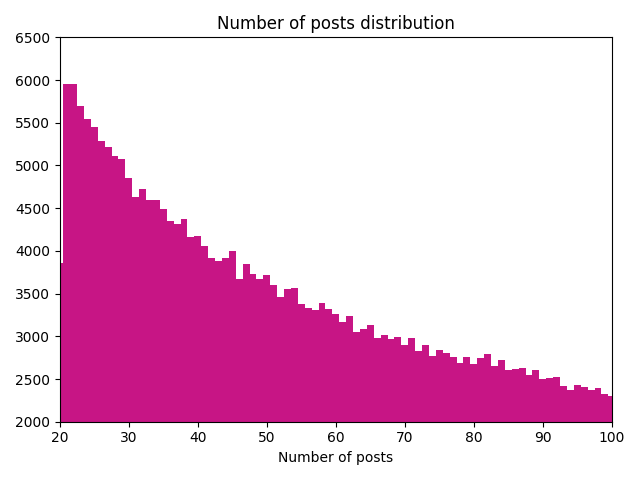
\includegraphics[width=0.55\textwidth]{data/pics/num_posts.png}
%\vspace*{-0.3cm}
\caption{Counts of users having $x$ number of Reddit posts.}
\label{num_posts}
\end{figure}

Almost 19K users in RedDust have two personal attributes known, 980 users have three and 28 have four attributes known,
which amounts to 6\% of the users having multiple personal attributes in total.
For  
such users
it is interesting to look at the interplay between different personal traits, for instance, the correlation between users' occupations and general interests.
In Figure \ref{prof-hob} we plot a heat map which represents the co-occurring values for these two predicates. 
For this experiment as well as the subsequent ones, we limit the number of professions and hobbies to the top $k$ ones ($k=20$ and $k=30$ for \textit{profession} and \textit{hobby}, respectively), sorted by the number of labeled users per value.

We observed intuitive correlations such as:
\emph{musicians} often play \emph{guitar};
\emph{runners} have \emph{running} as the main interest; 
\emph{college students} like to \emph{read} but are also interested in \emph{video games} five times as much as any other professions;
and curiously, \emph{shooting} is popular among \emph{photographers}, most probably because of \textit{shooting} being an ambiguous term.

\begin{figure*}[]
  \centering
  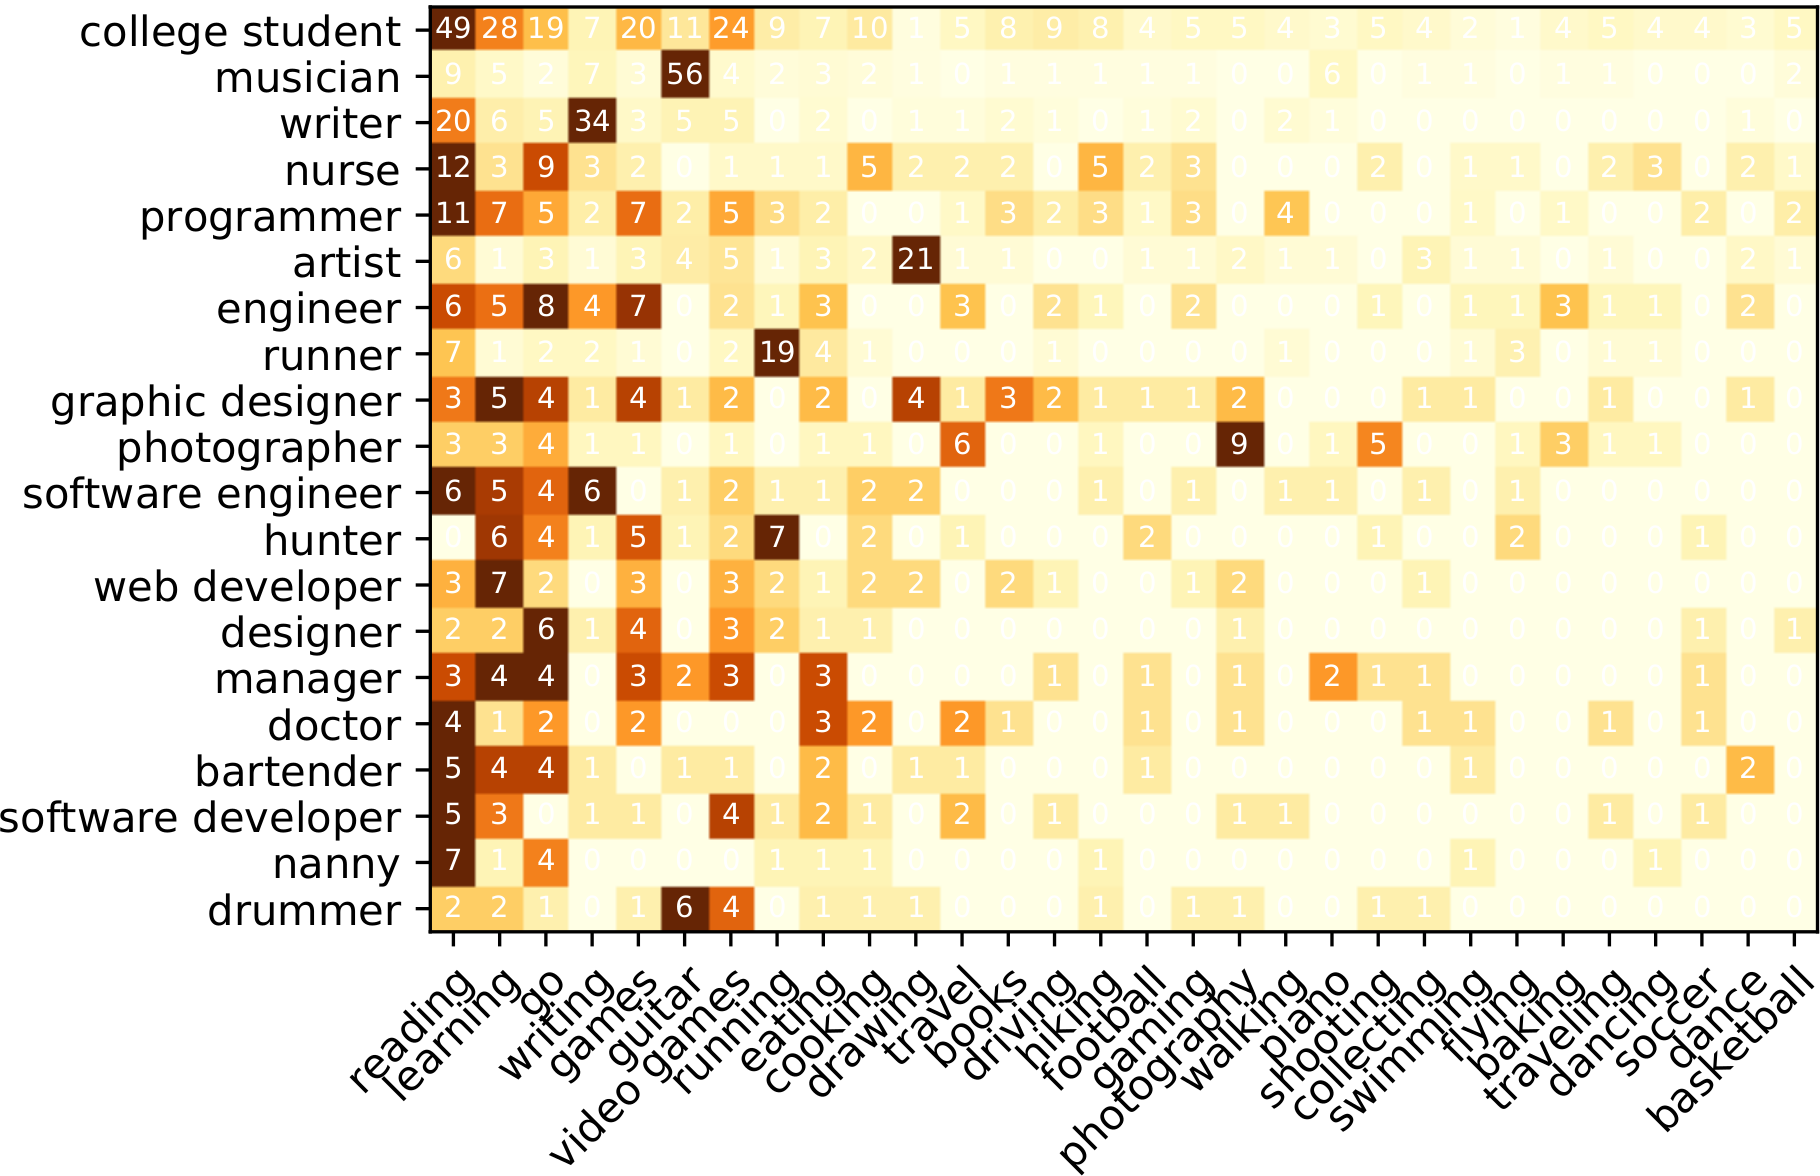
\includegraphics[width=0.77\linewidth]{data/pics/hob_prof.png}
  \caption{Co-occurrence of the most common professions and hobbies.}
  \label{prof-hob}
\end{figure*}

We also considered other pairs of attributes, namely \textit{profession} and \textit{gender}, for which we show the gender distribution of each profession in Figure \ref{prof_gender}. 
The analysis revealed common prejudices like \emph{female nannies} or \emph{male programmers},  
as well as several surprising insights (prevalence of \textit{female runners} and \textit{bartenders}) possibly specific to Reddit communities.

\begin{figure*}[]
\centering
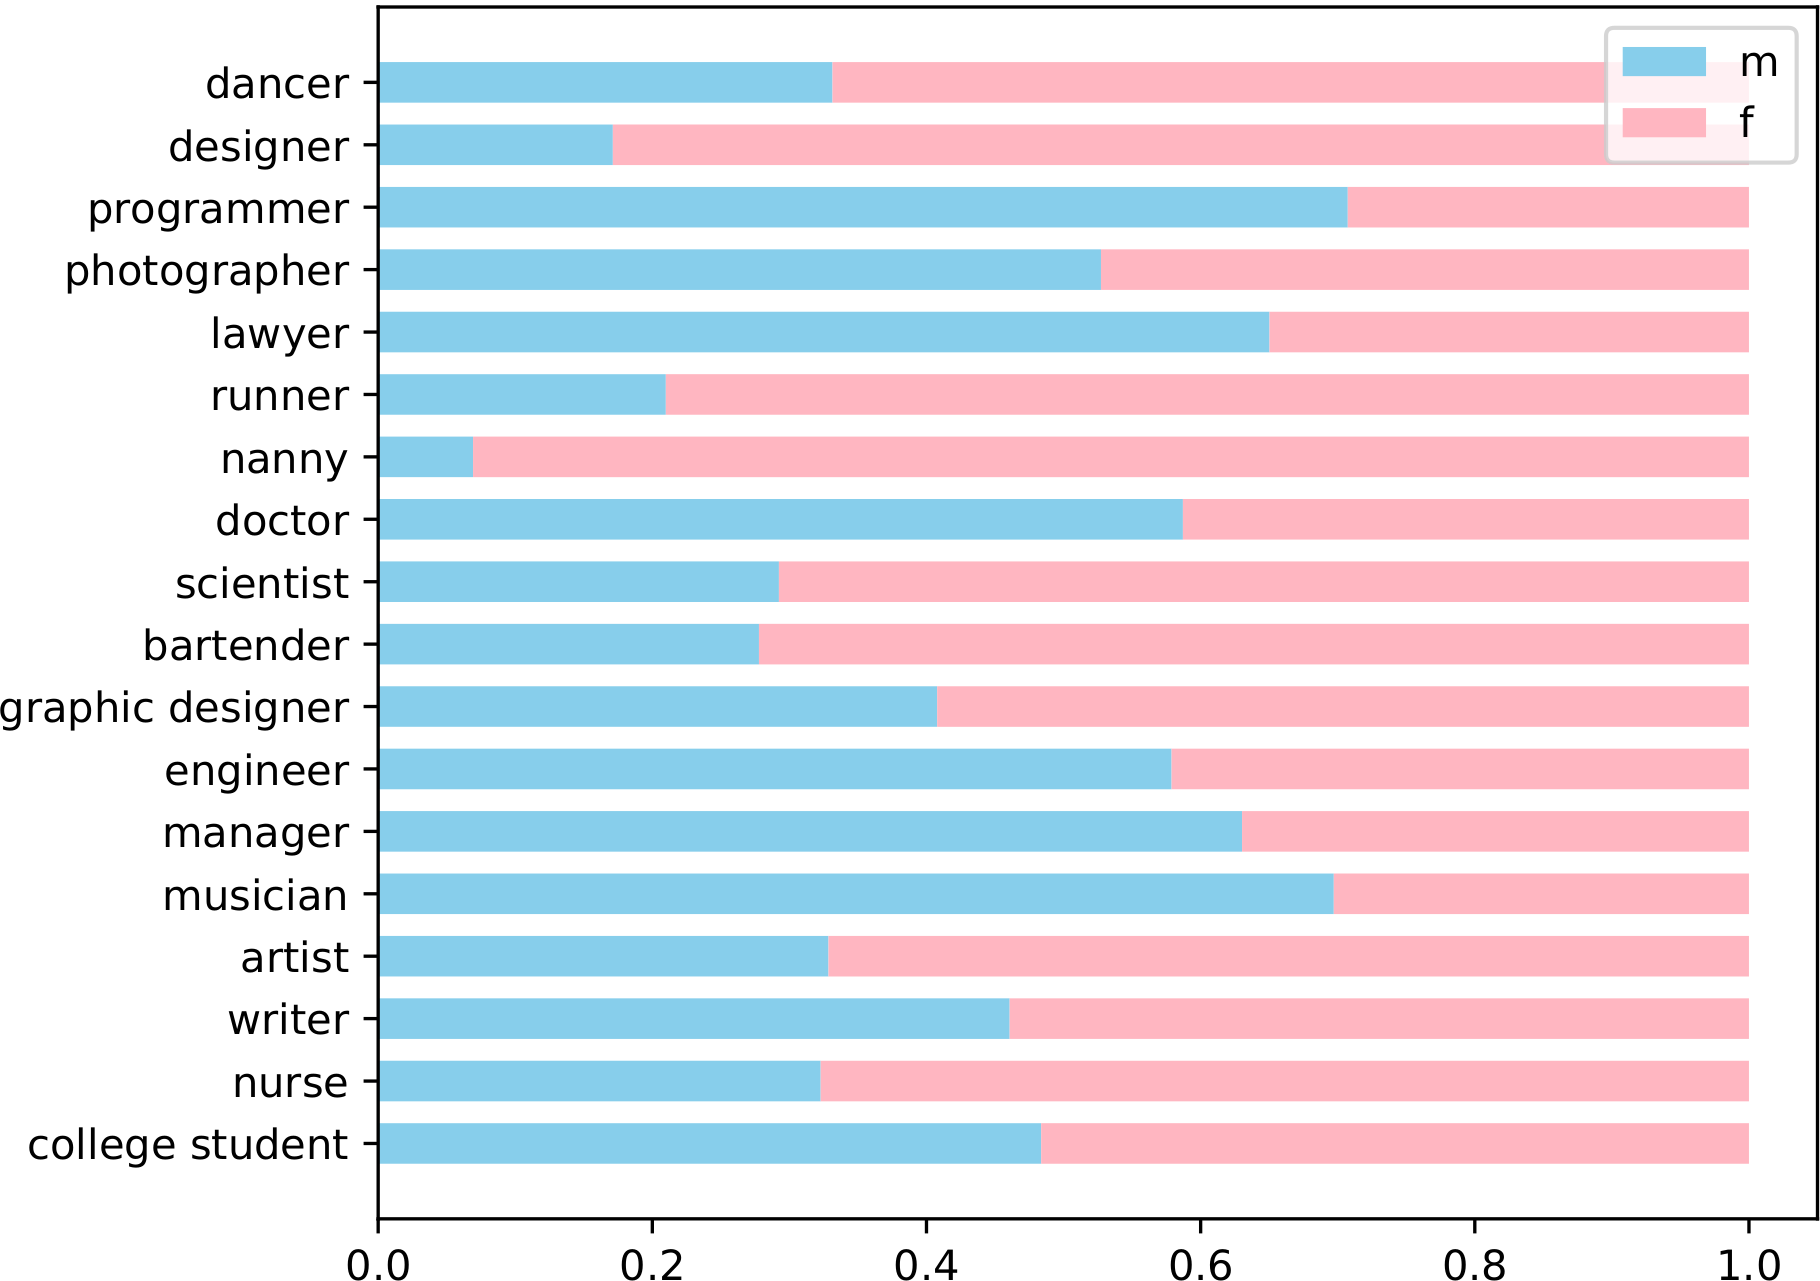
\includegraphics[width=0.67\linewidth]{data/pics/prof_gend.png}
\caption{Gender distribution among professions.}
\label{prof_gender}
\end{figure*}


\subsection{Labeling Reddit data with weak supervision}

While using explicit statements in brackets (e.g. [35f] indicating a \textit{35-year-old female}) and flairs is a reliable way to get age and gender of the users, utilizing natural language patterns (e.g. \textit{I am a doctor}) is a much nosier method, producing many false positive errors. In addition to that, the explicit assertions, required for the pattern-based approach are rare, because the users usually hint to their personal traits with subtler cues (for example, a profession \textit{doctor} can be deduced from the frequent use of medical terms in the posts). 

Keeping in mind these limitations of the natural language pattern-based approach we turn to the \textit{weak supervision} method to create a refined dataset for \textit{hobby} and \textit{profession} user traits. 

\paragraphHd{Snorkel.} We used the Snorkel framework \cite{ratner2017snorkel}, which allows data labeling using weak supervision. 
Snorkel does not require manual evaluation of each data sample, instead it relies on the outputs of multiple \textit{labeling functions}, such as patterns or heuristics, which are manually specified and can be potentially noisy. The accuracies and correlations of the labeling functions are then estimated by automatically deriving the \textit{generative model} over the labeling functions. The generative model weights and combines the outputs of labeling functions to produce final list of probabilistic labels.

\vspace{10pt}

We modified the criteria for including Reddit submissions, so that they are:
\emph{(1)} authored by users having 10-50 posts, \emph{(2)} 10-40 words long, and \emph{(3)} containing a personal pronoun (except for 3rd person ones).
Requirements \emph{(1)} and \emph{(2)} were derived from observing the word and post distributions on the full dataset.
Requirement \emph{(3)} comes from the assumption that posts containing personal pronouns are most likely to contain personal assertions. These restrictions allow us to select posts that look more similar to the real conversation (i.e., relatively short and containing references to the speakers with personal pronouns).
In addition, we did not consider the following subreddit types: \emph{(i)} \emph{dating}, which may provide plenty of personal information but no real conversation to infer from,
and \emph{(ii)} \emph{fantasy/video games} (for the \emph{profession} attribute), because users may refer to gaming personalities.
We selected only the users whose utterances contain at least one mention of the attribute values, from the Wikipedia lists of professions and hobbies,
resulting in around 250K and 500K candidate users for profession and hobby, respectively.

We then input the collected users into the Snorkel framework. Given a user's utterance set $U$, an attribute $a$ and a possible attribute value $v$, Snorkel will decide on a \emph{positive}/\emph{negative} label--denoting the user as having/not having personal trait~$a$~:~$v$; or if the decision can't be made -- an \emph{abstain} label.%, by combining multiple noisy outputs from the labeling functions with a probabilitsic model.

We have separate labeling models for each attribute $a$, and defined two labeling functions which consider: \emph{(LF1)} the existence of the \emph{attribute-specific patterns}, and \emph{(LF2)} the weighted count of the words belonging to the \emph{value-specific lexicon}.

\paragraphHd{LF1: Attribute-specific patterns.} We compiled a list of positive and negative patterns for each attribute (see Table \ref{tab:patterns}), e.g., \emph{``my hobby is $\langle$hobby-value$\rangle$''} vs \emph{``I hate $\langle$hobby-value$\rangle$''} as positive vs negative patterns for hobby.
LF1 labels a user with a \emph{positive/negative} label for each attribute value $v$ if there exist at least one positive/negative pattern in the user's utterances $U$, and \emph{abstain} otherwise.

\begin{table}[t!]
\centering
\small
\begin{adjustbox}{width=0.95\textwidth}
\begin{tabular}{@{}lllll@{}}
\toprule
\multicolumn{2}{c}{\textit{\textbf{profession}}} & \multicolumn{3}{c}{\textit{\textbf{hobby}}}                     \\ \midrule
\textbf{positive}       & \textbf{negative}      & \multicolumn{2}{c}{\textbf{positive}} & \textbf{negative}       \\ \midrule
 \begin{tabular}[t]{@{}l@{}} i am/i'm a(n)\\my profession is\\i work as\\my job is\\my occupation is\\i regret becoming a(n)  \end{tabular}                                                   & \begin{tabular}[t]{@{}l@{}} (no/not/don't \\within pos. patterns)  \end{tabular} 
 & \begin{tabular}[t]{@{}l@{}} i am/i'm obsessed with\\i am/i'm fond of\\i am/i'm keen on\\i like\\i enjoy\\i love\\i play\\i take joy in\\i adore\\i appreciate\\i am/i'm fan of \end{tabular}  
  & \begin{tabular}[t]{@{}l@{}} i am/i'm fascinated by\\i am/i'm interested in\\i fancy\\i am/i'm mad about\\i practise\\i am/i'm into\\i am/i'm sucker for \\ my interest is\\ my hobby is\\ my passion is\\ my obsession is \end{tabular}  
 &  \begin{tabular}[t]{@{}l@{}} i hate\\i dislike\\i detest\\i can't stand \\ (never/not/don't \\within pos. patterns) \end{tabular}  \\
\bottomrule
\end{tabular}
\end{adjustbox}
\caption{Positive and negative patterns used in the labeling function LF1 of the Snorkel labeling model. Each pattern must be followed by possible attribute values within a context window of 2 terms.}
\label{tab:patterns}
\end{table}


\paragraphHd{LF2: Value-specific lexicon.} For each attribute-value pair, we used \textit{Empath} \cite{fast2016empath} --pre-trained on the Reddit corpus-- to build a lexicon of \emph{typical words} (e.g., `cider' and `yeast' for \emph{hobby:brewing}). Given seed words, Empath builds lexical categories by means of an embedding model. As our value-specific lexicon, we took the union of Empath terms for a specific attribute value and all its synonyms; each typical word is weighted by embedding similarity to the seed words. 
Given a user's utterance set $U$ and an attribute value $v$, LF2 yields a \emph{positive} label if the weighted count of typical words of $v$ is above an empirically-chosen threshold, and \emph{abstain} otherwise.

\vspace{5pt}
Given a pair of user's utterance set $U$ and a possible attribute value $v$, the Snorkel probabilistic labeling model utilizes our labeling functions to
predict a confidence score for the \emph{positive} label, i.e., the user is labeled with attribute value $v$.
As our labeled dataset, we took only the user-value pairs with confidence scores above a specific threshold. 

To determine the threshold of confidence scores, we manually annotated a held-out validation set containing 100 users per attribute. 
Given a post and a set of attribute values mentioned explicitly in the post, the annotators had to identify whether the candidate user traits truly hold. For instance, from \emph{``My dad bought me a \textbf{chess} board even though I enjoy \textbf{video games} more''}, \emph{hobby:video games} is correct while \emph{hobby:chess} is not applicable.
The final annotation for each post consists of attribute values agreed by at least two out of three judges. The selected confidence threshold corresponds to the 0.9 precision of the model on the validation set. After thresholding, we obtained 13.5k users labeled with profession values and 11.7k users with hobby values.

To demonstrate that Snorkel provides the same level of quality as crowdsourcing,
we calculated the precision of human annotators
on the same validation set by comparing
the labels of each annotator against the agreement
labels. The obtained precision scores were 0.91 for
profession and 0.88 for hobby, demonstrating that
Snorkel is a reasonable alternative to crowdsourcing.



\subsection{Discussion}

Automatically labeling social media posts is an efficient and low-cost way to collect labeled conversations at scale. However, this approach only works for specific attributes (e.g. it is infeasible to collect \textit{relationships} among Reddit users, because most of them are strangers to each other). Another drawback of using social media platforms is the skewed user demographics distribution, such as prevalence of young people or several professions being underrepresented. Moreover, the labels obtained from pattern search are much noisier than the crowdsourced ones, requiring further manual revision steps. Finally, the attribute value lists automatically collected from Wikipedia can be further refined by merging redundant values and adding the missing ones.